% tutorial.tex  -  a short descriptive example of a LaTeX document
%
% For additional information see  Tim Love's ``Text Processing using LaTeX''
% http://www-h.eng.cam.ac.uk/help/tpl/textprocessing/
%
% You may also post questions to the newsgroup <b> comp.text.tex </b> 

\documentclass[12pt]{article}			% For LaTeX 2e
						% other documentclass options:
						% draft, fleqn, openbib, 12pt

\usepackage{graphicx}	 			% insert PostScript figures
\usepackage{caption}
\usepackage{subcaption}
\usepackage{wrapfig}
\usepackage{amsmath}
%% \usepackage{setspace}   % controllabel line spacing
%% If an increased spacing different from one-and-a-half or double spacing is
%% required then the spacing environment can be used.  The spacing environment 
%% takes one argument which is the baselinestretch to use,
%%         e.g., \begin{spacing}{2.5}  ...  \end{spacing}


% the following produces 1 inch margins all around with no header or footer
\topmargin	=10.mm		% beyond 25.mm
\oddsidemargin	=0.mm		% beyond 25.mm
\evensidemargin	=0.mm		% beyond 25.mm
\headheight	=0.mm
\headsep	=0.mm
\textheight	=220.mm
\textwidth	=165.mm
					% SOME USEFUL OPTIONS:
% \pagestyle{empty}			% no page numbers
 \parindent  15.mm			% indent paragraph by this much
 \parskip     2.mm			% space between paragraphs
% \mathindent 20.mm			% indent math equations by this much

\newcommand{\MyTabs}{ \hspace*{25.mm} \= \hspace*{25.mm} \= \hspace*{25.mm} \= \hspace*{25.mm} \= \hspace*{25.mm} \= \hspace*{25.mm} \kill }

\graphicspath{{../Figures/}{../data/:}}  % post-script figures here or in /.

					% Helps LaTeX put figures where YOU want
 \renewcommand{\topfraction}{0.9}	% 90% of page top can be a float
 \renewcommand{\bottomfraction}{0.9}	% 90% of page bottom can be a float
 \renewcommand{\textfraction}{0.1}	% only 10% of page must to be text

\linespread{1.2}
\alph{footnote}				% make title footnotes alpha-numeric

\title{Continuous Multimodal User Authentication, using hard and soft biometric traits}	% the document title
\author{{\bf Project report}{\bf}}
\date{}				% your own text, a date, or \today

% --------------------- end of the preamble ---------------------------

\begin{document}			% REQUIRED

\pagenumbering{roman}			% Roman numerals from abstract to text
\maketitle				% you need to define \title{..}
\thispagestyle{empty}			% no page number on THIS page 

\begin{center}

%A synopsis submitted in partial fulfillment of the requirements of the course \\[3ex]
{\Large CS812}\\[3ex]
{\Large}

{\large}
{\bf Under the guidance of }{\bf}\\[2ex]
Dr. K. G. Srinivasa\\
Professor\\
Department of Computer Science and Engineering\\
M. S. Ramaiah Institute of Technology\\[3ex]


{\bf Submitted by}{\bf}\\[2ex]
{\bf Soumya Gosukonda }{\bf} 1MS08CS119\\
{\bf Tribhuvanesh Orekondy }{\bf} 1MS08CS129\\[8ex]
{\large}


\includegraphics[scale=0.20]{msrit.png}\\
Department of Computer Science and Engineering\\
M. S. Ramaiah Institute of Technology\\
(Autonomous Institute Affiliated to VTU)\\
Bangalore - 560054
\end{center}

\newpage
\begin{abstract}			% beginning of the abstract

% TODO <-----ABSTRACT GOES HERE------>

Password based security is a commonly used measure to enforce valid authentication. Coupled with Iris and/or fingerprint based recognition, these systems, known as biometric authentication systems, strengthen this process of authentication. However, this is a one-time process and fails to provide continuous authentication. To illustrate the idea of Continuous Authentication (CA) consider a situation where the user has to leave her/his workstation unattended for a short period of time and forgets to lock it. In this time interval it is possible for an unauthorized user to gain access to the system and tamper with it. To avoid such a situation, continuous authentication can prove useful. 
This project aims to deliver a continuous authentication system based on face recognition and soft biometric traits, namely shirt colour. We plan to achieve this goal using the OpenCV library and a suitable mathematical model.


\end{abstract}				% end of the abstract
\newpage
\begin{center}
{\LARGE \bf Acknowledgements}
\\[6ex]
\end{center}
We would like to thank our project guide, Dr. K.G.Srinivasa, for his valuable and much-needed guidance and patience during the course of this project. We are grateful for the timely inputs we received from him, right from the start of the project.\\[2ex]
We are thankful to the Department of Computer Science and Engineering, and our Head of Department, Dr. R. Selvarani, for having provided us an opportunity to work on this project and enhance our skills in this field.\\[2ex]
We also thank the lab assistants and our friends for their immense help and suggestions that helped us further improve the project. 
\newpage				% start a new page
\tableofcontents			% create table of contents automatically
\newpage				% start a new page
\pagenumbering{arabic}			% Arabic page numbers from now on

\section{ Introduction }	% start the first numbered section

% <-------- INTRODUCTION -------->

\subsection{ General Introduction }
Over the years, \emph{static authentication} - the procedure of allowing user access based on one-time authentication, has evolved from using passwords to more modern and technologically advanced methods such as finger-print based systems and iris recognition. Google accounts use a phone-verification method in which the user after a conventional password login, is immediately sent a passcode to his/her phone which needs to be entered to gain access to the account.\\
These methods, although providing a rigid and secure framework to this one-time authentication, doesn't authenticate the user throughout the session. This leaves the possibility of an imposter gaining access in multiple scenarios. Below are few examples,
\begin{itemize}
\item The authenticated user takes a short-break without logging-out, and an imposter takes his place  and is allowed all the privileges that existed to the authenticated user
\item The authenticated user is coerced by an attacker to enter his credentials and hence gain subsequent access.
\item Softwares such as iTunes, Google Play store or the Kindle store on mobile devices, contains pre-authorized credit-card information to enable instant purchases. When an attacker gains access to such systems, he can make fradulent or unnecessary purchases and leave no trace of his identity behind.
\end{itemize}
\emph{Continuous Authentication} hence provides a solution by authenticating the user right from the initial stages of log-in through log-out. This is implemented by checking the hard biometric traits (eg, facial features) of the user during log-in and his/hew soft biometric traits\cite{Niin10}(eg, such as colour of the user's clothing, complexion, etc.)\\
The multiple modes refer to the system's ability to use hard biometric traits and soft biometric traits, and switch between the two to maintain a certain level of confidence. 

\subsection{ Statement of the Problem }
Soft biometric traits don't provide as high a level of confidence as hard biometric traits. \cite{Niin10} suggests using these soft-biometric traits throughout the authenticated period to provide high tolerance to the user's posture in front of the computer system. Albeit, this being true as shown in our experiments, the problem is to incorporate both traits during the authenticated period, switching between them as and when necessary, depending on the confidence calculated using an appropriate mathematical model. \\
Hard biometric traits, which in this case is face recognition using Eigenfaces\cite{Turk91} is used over its counterparts, such as iris and fingerprint based recognition, since these options are not only expensive, but also cannot be used during the authenticated session without interrupting the user from his work-flow. Thw disadvantage of solely running on face recognition lies in the fact that its computationally expensive and posture-dependent. The problem hence extends to take into account these factors when building the system.

\subsection{ Objectives of the Project }
With the statement of the problem as described earlier, this objectives of tis project can be tersely stated as follows:
\begin{itemize}
\item A low-cost solution with the user not compelled to invest in expensive or extra hardware.
\item Incorporating techniques to intelligently authenticate the user throughout the session, by logging-in using conventional and the time-tested method of a one-time password based
\item The one-time password based authentication step to be followed by analyzing the unique-per-user hard biometric traits to achieve a high level of confidence and proceed to soft-biometric measures to maintain that confidence
\item Instead of bifurcating the hard and soft biometric authentication phases into clearly distinct phases as suggested by \cite{Niin10}, using a suitable model to shift between the two phases and maintain that level of confidence without the user's work-flow being interrupted unless there exists a large uncertainity
\item To allow the theory to be extended to include more modalities
\end{itemize}

% \subsection{ Current scope }
% The current scope of this project is tp have the multimodal continuous authentication system installed on a local machine, with technical specifications on par with an average system available in the current market. The system proceeds with Face Recognition using Eigenfaces\cite{Turk91} to capture the unique-per-person hard biometric traits and the user's shirt colour for the soft biometric traits.

\newpage

\section{Literature Survey }
\subsection{ Authentication }
Authentication is the process of verifying the claimed identity of a user. The network elements
(NE) environment must offer features to verify the claimed identity of a user before giving that
user operations access. Depending on the NE and the applications, there could be different kinds
of authenticators. For example according to \cite{war02}
\begin{itemize}
\item The user can be associated with confidential information that only he or she is supposed
to posses such as: password, private key, or randomly time-varying PIN (such as those
provided by single-use password tokens)
\item The user can be associated with a distinctive physical or logical address (e.g., user’s
authorized directory number, network address)
\item The user can be authenticated by certain unique attributes such as: voice or speech
pattern, handwriting style, palm print, or retina scan.
\end{itemize}
There are three fundamental techniques used in authentication mechanisms\cite{john03}
\begin{itemize}
\item Something you know, which usually refers to passwords and PINs. The simplest
implementations of passwords and personal identification numbers (PINs) yield the
simplest of all authentication mechanisms.
\item Something you have, which usually refers to cards or tokens. Physical authentication
devices, such as smart cards and password tokens, were developed to eliminate certain
weakness associated with passwords. A major benefit of cards and tokens is that they
can’t be shared with the same freedom as sharing passwords.
\item Something you are, which refers to biometrics - the measurement of physical
characteristics or personal traits. Common biometric verification techniques try to match
measurements from one user’s fingerprint, hand, eyes, face, or voice to measurements that
were previously collected from him/her.
\end{itemize}
There are two general applications for this: identification and verification. “With identification,
the biometric system asks and attempts to answer the question, ‘who is X?’ Verification occurs
when the biometric system asks and attempts to answer the question, ‘is this X?’ after the user
claims to be X. In a verification application, the biometric system requires input from the user, at
which time the user claims his or her identity via a password, token, or user name. This user input
points the system to a template in the database. The system also requires a biometric sample from
the user. It then processes and compares the sample to or against the user. This is called a “one-
to-one search (1:1)”

\subsection{ Authentication methods }
All methods of authentication require you to specify who or what you are and to relay appropriate
credentials to prove that you are who you say you are. These credentials generally take the form
of something you know, something you have, or something you are. What you know may be a
password. What you have could be a smart card. What you are pertains to the field of biometrics.
The important element is to recognize that different mechanisms provide
authentication services with varying degrees of certainty. Choosing the proper authentication
technology largely depends on the location of the entities being authenticated and the degree of
trust placed in the particular facets of the network.\\
The following sections delve into key methods used in this project.

\subsubsection{ Username and Password authentication }
Username and password are often used in the practical world. It’s a method which is based on “what you know” for authentication.
It is the simplest way of authentication and it provides each user with a unique username and a
secret password. It is an easy way to get attacked by password guessing. As long as a user can enter the correct username and password, the
computer and system will assume that the operator who using the computer is the legal user or original user.

\subsubsection{ Biometrics }
Biometrics is first introduced in the 1970s and early 1980s. This technology gathers unique
physiological or behavioral attributes of a person for storing in a database or comparing it with
data already found in the database. Same as test procedure reference, a biometric is \emph{“defined as a
unique, measurable, biological characteristic or trait for automatically recognizing or verifying
the identity of a human being. Statistically analyzing these biological characteristics has become
known as the science of biometrics.”} These days, biometric technologies are typically
used to analyze human characteristics for security purposes. Five of the most common physical
biometric patterns analyzed for security purposes are fingerprint, hand, eye, face, and voice.\\
Biometrics, can in our case, be classified into \emph{Hard Biometric traits}, which remain unique-per-user and
\emph{Soft Biometric traits}, which remain unique-per-session.

\subsubsection{ Hard Biometrics}

\subsubsection{ Soft Biometrics }
The first personal identification system developed by Alphonse Bertillon\cite{bert96} for identification of criminals was based
on three sets of features: (i) body measurements (anthropometry) like height and length of the arm, (ii) morphological
description of the appearance and shape of the body like eye color and anomalies of the fingers, and (iii) peculiar marks
observed on the body like moles, scars, and tattoos. Although the Bertillon system was very useful in tracking crimi-
nals, it had an unacceptably high rate of false identification. This was due to two reasons. Firstly, several individuals
can have the same set of values for these measurements. Secondly, for the same individual, these values can change
over time. In other words, these characteristics do not have the distinctiveness and permanence to uniquely identify
an individual over a period of time and hence we refer them as soft biometric traits. {\bf \it Soft biometric traits are those
characteristics that provide some information about the individual, but lack the distinctiveness and permanence to
sufficiently differentiate any two individuals.}\cite{Jain204}\\
The soft biometric traits can either be continuous or discrete. Traits such as gender, eye color, ethnicity, etc. are discrete in nature. On
the other hand, traits like height and weight are continuous variables. A system that is completely based on soft bio-
metric traits cannot provide the required accuracy in the recognition of individuals.\\
Wayman\cite{way97} proposed the use of soft biometric traits like gender and age, for filtering a large biometric database.
Filtering refers to limiting the number of entries in a database to be searched, based on characteristics of the interacting
user. For example, if the user can somehow be identified as a middle-aged male, the search can be restricted only to
the subjects with this profile enrolled in the database. This greatly improves the speed or the search efficiency of
the biometric system. Filtering reduces the probability of obtaining a wrong match, but this is offset by the fact that
the errors in filtering also reduce the probability of obtaining a correct match. Hence, in general, filtering drastically
reduces the time required for identification but can degrade the recognition performance.


\subsection{ Continuous Authentication Systems }
\begin{figure}
	\centering
		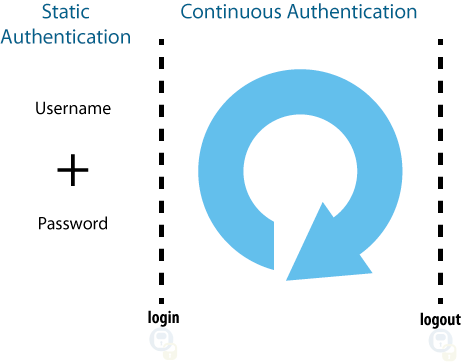
\includegraphics[scale=0.6]{img/ca1.png}
	\caption{Continuous Authentication}
\end{figure}
Continuous Authentication system have gained momentum over the recent years due to the advancement in technology to handle computationally expensive tasks, as well as the need to secure the vast amount of private information that can be exchanged during an authenticated session.\\
Various studies\cite{mon00,turk03,sim07,azz08,azz082,kang06,car03} have been carried out on the problem of Continuous Authentication.
Sensible Vision's \emph{Fast Access} provides an industrial solution, with the solution involving a proprietay set-up and being paid.

\subsection{ Face Detection }
OpenCV's face detector uses a method that Paul Viola and Michael Jones published in 2001\cite{Viola01}. Usually simply called the Viola-Jones method, or even just Viola-Jones, this approach to detecting objects in images combines four key concepts that can be summarized the four key-steps.
\begin{itemize}
	\item Simple rectangular features, called Haar features
	\item An Integral Image for rapid feature detection
	\item The AdaBoost machine-learning method
	\item A cascaded classifier to combine many features efficiently
\end{itemize}
\begin{figure}
	\centering
	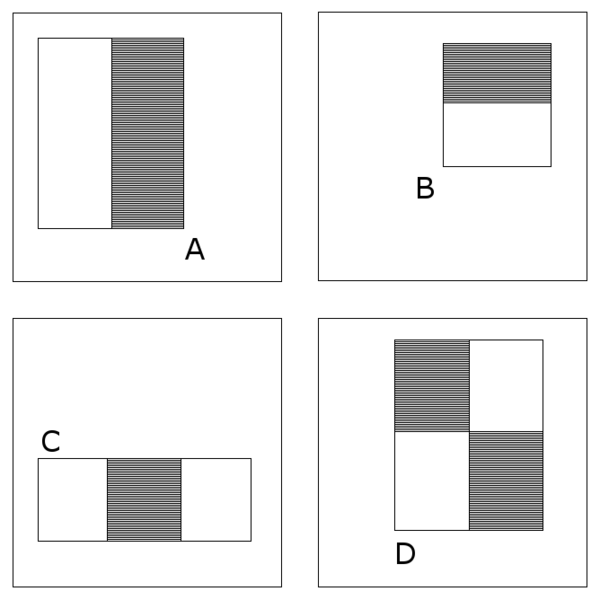
\includegraphics[scale=0.3]{img/fd5.png}
	\caption{Examples of Haar features in OpenCV}
	\label{fig:fd1}
\end{figure}
The features that Viola and Jones used are based on Haar wavelets. Haar wavelets are single wavelength square waves (one high interval and one low interval). In two dimensions, a square wave is a pair of adjacent rectangles - one light and one dark.\\
The actual rectangle combinations used for visual object detection are not true Haar wavlets. Instead, they contain rectangle combinations better suited to visual recognition tasks. Because of that difference, these features are called Haar features, or Haarlike features, rather than Haar wavelets. Figure \ref{fig:fd1} shows the features that OpenCV uses.The presence of a Haar feature is determined by subtracting the average dark-region pixel value from the average light-region pixel value. If the difference is above a threshold (set during learning), that feature is said to be present.\\
To determine the presence or absence of hundreds of Haar features at every image location and at several scales efficiently, Viola and Jones used a technique called an Integral Image. In general, "integrating" means adding small units together. In this case, the small units are pixel values. The integral value for each pixel is the sum of all the pixels above it and to its left. Starting at the top left and traversing to the right and down, the entire image can be integrated with a few integer operations per pixel.\\
\begin{figure}[h!]
	\centering
	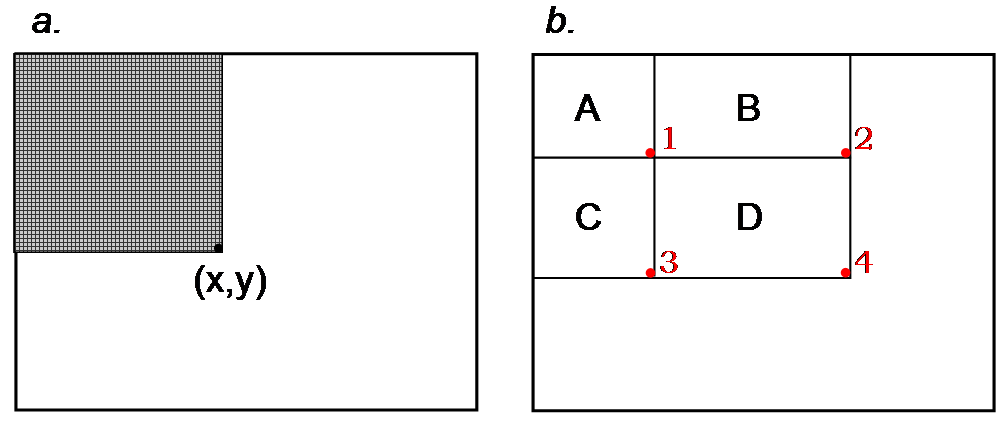
\includegraphics[scale=0.3]{img/fd3.png}
	\caption{The Integral Image trick}
	\label{fig:fd2}
\end{figure}
As Figure \ref{fig:fd2} shows, after integration, the value at each pixel location, (x,y), contains the sum of all pixel values within a rectangular region that has one corner at the top left of the image and the other at location (x,y). To find the average pixel value in this rectangle, you'd only need to divide the value at (x,y) by the rectangle's area.\\
But what if you want to know the summed values for some other rectangle, one that doesn't have one corner at the upper left of the image? Figure 2b shows the solution to that problem. Suppose you want the summed values in $D$. You can think of that as being the sum of pixel values in the combined rectangle, $A+B+C+D$, minus the sums in rectangles $A+B$ and $A+C$, plus the sum of pixel values in $A$. In other words,
\begin{center}
  $D = A+B+C+D -  (A+B) -  (A+C) + A$
\end{center}
Conveniently, $A+B+C+D$ is the Integral Image's value at location 4, $A+B$ is the value at location 2, $A+C$ is the value at location 3, and $A$ is the value at location 1. So, with an Integral Image, you can find the sum of pixel values for any rectangle in the original image with just three integer operations:
\begin{center}
\(
\left(x4, y4\right) - \left(x2, y2\right) - \left(x3, y3\right) + \left(x1, y1\right)
\).
\end{center}
To select the specific Haar features to use, and to set threshold levels, Viola and Jones use a machine-learning method called AdaBoost. AdaBoost combines many "weak" classifiers to create one "strong" classifier. "Weak" here means the classifier only gets the right answer a little more often than random guessing would. That's not very good. But if you had a whole lot of these weak classifiers, and each one "pushed" the final answer a little bit in the right direction, you'd have a strong, combined force for arriving at the correct solution. AdaBoost selects a set of weak classifiers to combine and assigns a weight to each. This weighted combination is the strong classifier.\\
\begin{figure}[h]
	\centering
	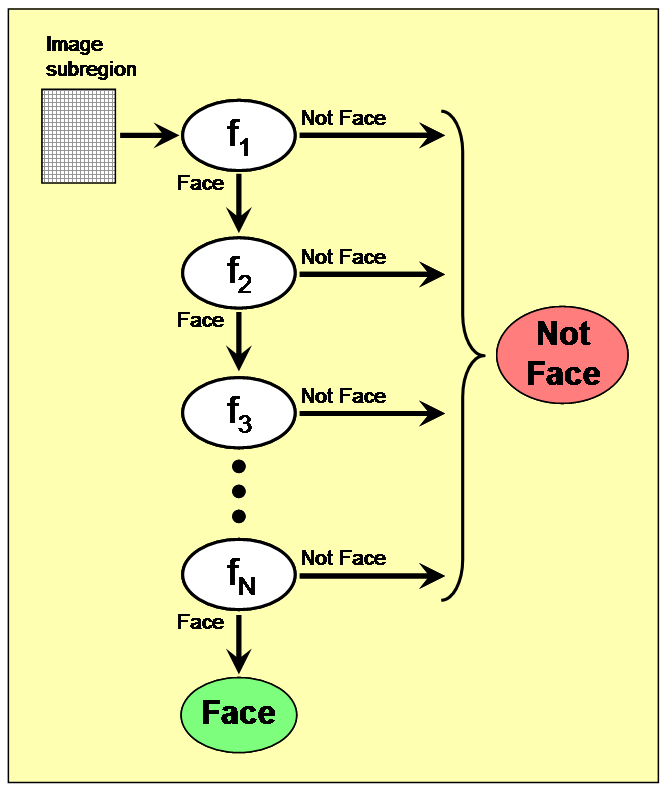
\includegraphics[scale=0.4]{img/fd4.png}
	\caption{\small The classifier cascade is a chain of filters. Image subregions that make it through the entire cascade are classified as "Face." All others are classified as "Not Face."}
	\label{fig:fd3}
\end{figure}
Viola and Jones combined a series of AdaBoost classifiers as a filter chain, shown in Figure \ref{fig:fd3}, that's especially efficient for classifying image regions. Each filter is a separate AdaBoost classifier with a fairly small number of weak classifiers.\\
The acceptance threshold at each level is set low enough to pass all, or nearly all, face examples in the training set. The filters at each level are trained to classifiy training images that passed all previous stages. (The training set is a large database of faces, maybe a thousand or so.) During use, if any one of these filters fails to pass an image region, that region is immediately classified as "Not Face." When a filter passes an image region, it goes to the next filter in the chain. Image regions that pass through all filters in the chain are classified as "Face." Viola and Jones dubbed this filtering chain a cascade.\\
The order of filters in the cascade is based on the importance weighting that AdaBoost assigns. The more heavily weighted filters come first, to eliminate non-face image regions as quickly as possible. Figure 4 shows the first two features from the original Viola-Jones cascade superimposed on my face. The first one keys off the cheek area being lighter than the eye region. The second uses the fact that the bridge of the nose is lighter than the eyes.


\subsection{ Face recognition using Eigenfaces }
Eigenfaces are a set of eigenvectors used in the computer vision problem of human face recognition. The approach of using eigenfaces for recognition was developed by Sirovich and Kirby (1987) and used by Matthew Turk and Alex Pentland in face classification\cite{Turk91}. It is considered the first successful example of facial recognition technology. These eigenvectors are derived from the covariance matrix of the probability distribution of the high-dimensional vector space of possible faces of human beings.\\

\subsubsection{ Eigenface generation }
A set of eigenfaces can be generated by performing a mathematical process called principal component analysis (PCA) on a large set of images depicting different human faces. Informally, eigenfaces can be considered a set of "standardized face ingredients", derived from statistical analysis of many pictures of faces. Any human face can be considered to be a combination of these standard faces. For example, one's face might be composed of the average face plus 10\% from eigenface 1, 55\% from eigenface 2, and even -3\% from eigenface 3. Remarkably, it does not take many eigenfaces combined together to achieve a fair approximation of most faces. Also, because a person's face is not recorded by a digital photograph, but instead as just a list of values (one value for each eigenface in the database used), much less space is taken for each person's face.\\

The eigenfaces that are created will appear as light and dark areas that are arranged in a specific pattern. This pattern is how different features of a face are singled out to be evaluated and scored. There will be a pattern to evaluate symmetry, if there is any style of facial hair, where the hairline is, or evaluate the size of the nose or mouth. Other eigenfaces have patterns that are less simple to identify, and the image of the eigenface may look very little like a face.\\

The technique used in creating eigenfaces and using them for recognition is also used outside of facial recognition. This technique is also used for handwriting analysis, lip reading, voice recognition, sign language/hand gestures interpretation and medical imaging analysis. Therefore, some do not use the term eigenface, but prefer to use 'eigenimage'.\\[2ex]
{\bf Implementation}\\
To create a set of eigenfaces, one must:
\begin{enumerate}
\item Prepare a training set of face images. The pictures constituting the training set should have been taken under the same lighting conditions, and must be normalized to have the eyes and mouths aligned across all images. They must also be all resampled to a common pixel resolution $(r \times c)$. Each image is treated as one vector, simply by concatenating the rows of pixels in the original image, resulting in a single row with $r \times c$ elements. For this implementation, it is assumed that all images of the training set are stored in a single matrix T, where each row of the matrix is an image.

\item Subtract the mean. The average image a has to be calculated and then subtracted from each original image in T.

\item Calculate the eigenvectors and eigenvalues of the covariance matrix S. Each eigenvector has the same dimensionality (number of components) as the original images, and thus can itself be seen as an image. The eigenvectors of this covariance matrix are therefore called eigenfaces. They are the directions in which the images differ from the mean image. Usually this will be a computationally expensive step (if at all possible), but the practical applicability of eigenfaces stems from the possibility to compute the eigenvectors of S efficiently, without ever computing S explicitly, as detailed below.

\item Choose the principal components. The $D \times D$ covariance matrix will result in D eigenvectors, each representing a direction in the $r \times c$-dimensional image space. The eigenvectors (eigenfaces) with largest associated eigenvalue are kept.
\end{enumerate}
These eigenfaces can now be used to represent both existing and new faces: we can project a new (mean-subtracted) image on the eigenfaces and thereby record how that new face differs from the mean face. The eigenvalues associated with each eigenface represent how much the images in the training set vary from the mean image in that direction. We lose information by projecting the image on a subset of the eigenvectors, but we minimize this loss by keeping those eigenfaces with the largest eigenvalues. For instance, if we are working with a 100 x 100 image, then we will obtain 10,000 eigenvectors. In practical applications, most faces can typically be identified using a projection on between 100 and 150 eigenfaces, so that most of the 10,000 eigenvectors can be discarded.\\

\noindent{\bf Computing Eigenvectors}

Performing PCA directly on the covariance matrix of the images is often computationally infeasible. If small, say 100 x 100, greyscale images are used, each image is a point in a 10,000-dimensional space and the covariance matrix S is a matrix of 10,000 x 10,000 = 108 elements. However the rank of the covariance matrix is limited by the number of training examples: if there are N training examples, there will be at most N-1 eigenvectors with non-zero eigenvalues. If the number of training examples is smaller than the dimensionality of the images, the principal components can be computed more easily as follows.

Let {\bf T} be the matrix of preprocessed training examples, where each column contains one mean-subtracted image. The covariance matrix can then be computed as {\bf S = T$^{T}$T} and the eigenvector decomposition of {\bf S} is given by\\
\begin{align*}
Sv_{i} = TT^{T}v_{i} = \lambda_{i}v_{i}
\end{align*}
However {\bf T$^{T}$T } is a large matrix, and if instead we take the eigenvalue decomposition of
\begin{align*}
T^{T}Tu_{i} = \lambda_{i}u_{i}
\end{align*}
then we notice that by pre-multiplying both sides of the equation with {\bf T}, we obtain
\begin{align*}
TT^{T}Tu_{i} = \lambda_{i}Tu_{i}
\end{align*}
\newpage
\section{Software Requirements Specification }
\subsection{ Introduction }

\subsubsection{ Purpose }
The purpose of this Software Requirements Specification is to provide a complete description of all the specifications and functions of the Continuous Authentication system as described above.

\subsubsection{ Scope of the Project }
Continuous authentication prevents the system from compromising the user's authenticity by continuously ensuring that the confidence in the identity of the user doesn't fall below a certain threshold. A video-feed from the web-cam is used to capture the user's traits throughout the session. A session here can be associated with the user logged-in to an e-mail or online banking account, or an account on the operating system itself.

\subsubsection{ Overview of Document }
The rest of this Software Requirements Specification proceeds with a general description of the project followed by the specific requirements of this software. 

\subsection{ General Description }
\subsubsection{ Project Perspective }
The Continuous Authentication system is designed as a stand-alone application which grants the user certain privileges at the time of successful log-in and continuously authenticates the user. The application enters into a lock-down mode in case an unauthorized  user attempts to use the authenticated user's privileges. 

\subsubsection{ Product Functions }
The Continuous Authentication system aims to provide the two primary functions:
\begin{itemize}
	\item To check the hard biometric traits of the user during the initial log-in stage and during certain periods after log-in till session ends.
	\item Continuously monitor the identity of the authenticated user and lock-down when required.
\end{itemize}

\subsubsection{ End users }
This application provides an added layer of security for users who wish to protect access to confidential information. Consequently, the user can rely on the system to ensure the privacy of his/her information.

\subsubsection{ General Constraints }
This application is constrained by the following:
\begin{itemize}
	\item The end-user's system should be capable of processing the real-time video-feed.
	\item The lighting conditions during usage to be similar to that captured by the training set.
	\item The system is incapable of performing a hard biometric recognition in case of occlusion.
\end{itemize}

\subsubsection{ Assumptions and Dependencies }
This application is assumes the following:
\begin{itemize}
	\item The user's system is equipped with a web-cam.
	\item The user is working in a sufficiently illuminated environment.
\end{itemize}

\subsection{ Specific Requirements }
\subsubsection{ Functional Requirements }
\begin{itemize}
	\item{\it Provide initial log-in, and verify user's password followed by the user's hard biometric traits. }
	\item{\it Create an account for a new user in the xml database and collect user's facial features and retrain the model. }
	\item{\it Create a user template with the user's soft biometric traits (shirt colour) once the user's face has been recognized with a minimum given confidence level.  }
	\item{\it Use the shirt-colour template to continuously verify the user's identity.  }
	\item{\it If the soft biometric verification falls below a certain threshold, restart face recognition of the user.  }
	\item{\it Lock-down in case of a tailgating unauthorized user. }
	%\item{\it A session time-out occurs in case the user logs in and then leaves the workstation unattended for a specified time limit. }
\end{itemize}

\subsubsection{ Software Requirements }
\begin{itemize}
\item C++ compiler (g++ 4.6.1)
\item OpenCV libraries
\item Drivers for web-cam
\item Python 2.7.1
\end{itemize}

\subsubsection{ Hardware Requirements }
\begin{itemize}
\item Web-cam with drivers supported by OpenCV, with a minimum resolution of 1.3MP
\item Memory : 2GB DDR2
\item Processor : A minimum of 3.0GhZ single core processor
\end{itemize}

\subsection{ Interface Requirements }
\subsubsection{ User Interface }
The user interface is provided with functions necessary to take as input the credentials of the user and display the live video-feed from the web-cam.

\section{ System Architecture and Design }  
\subsection{ Block diagram }
\begin{center}
    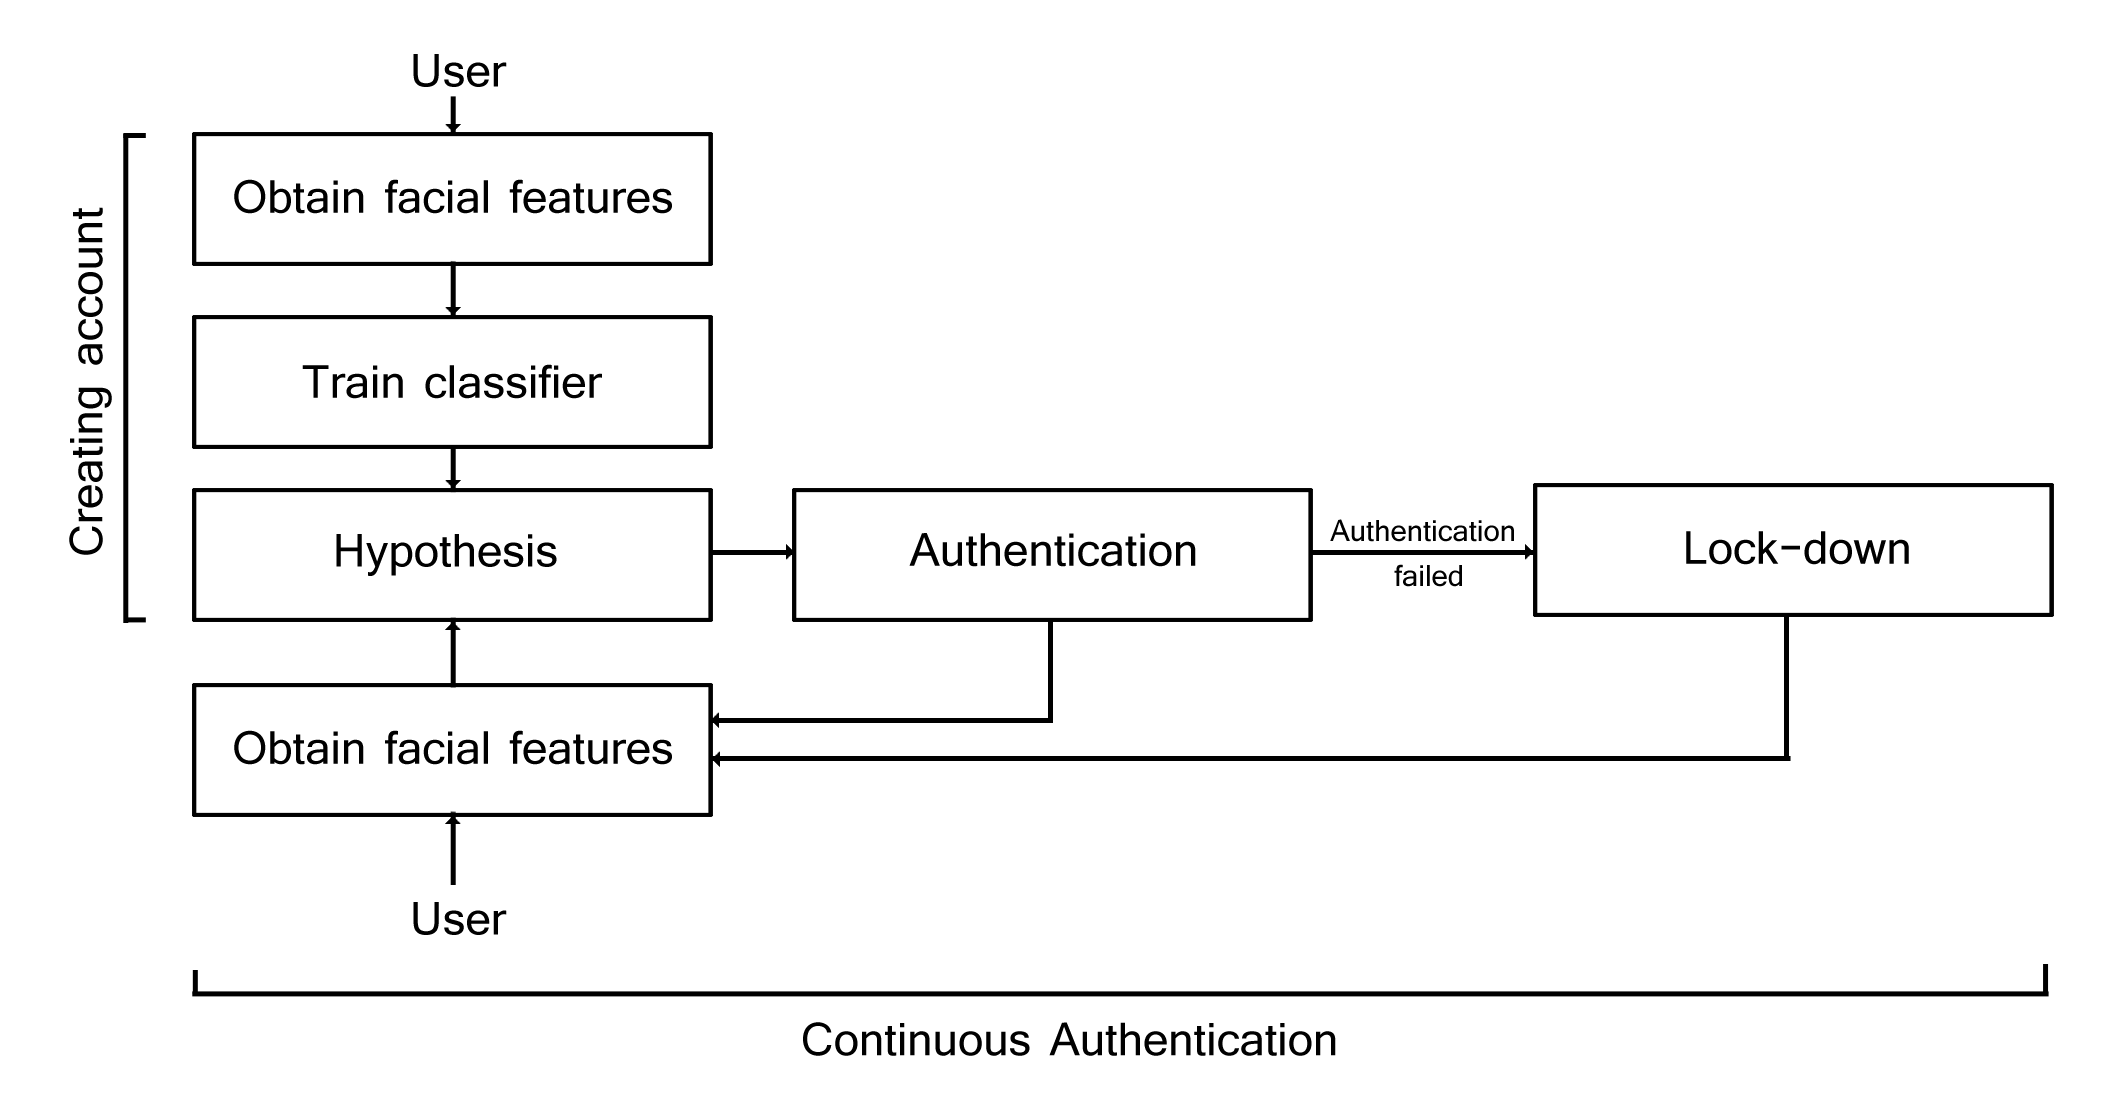
\includegraphics[scale=0.8]{block.png}
\end{center}

\section{ Detailed Design }
\subsection{ Data Persistence }
The persistent data in this system consists of:
\begin{itemize}
\item Training data set - Training data set consists of 51 equalized, grayscale images of each user stored in their respective directories. These are collected from a web-cam when a new user creates an account.% TO MENTION - resolution of pics
\item Eigenfaces data - This training data set is used to compute, using Principal Component Analysis, a set of "EigenFaces" representing the main differences between the training images. An "average face image" is computed and stored as \verb+avg_image.jpeg+. 
\item User-account data - User-account data refers to user-id, username, password stored in the form of a 160-bit hash string (SHA-1 encrypted).
\end{itemize}

An XML file names \verb+"face_data.xml"+ contains the integrated eigenfaces and user-account data. Its structure is as shown below:
\begin{verbatim}
-<opencv_storage>
	<nPersons>number of users</nPersons>
	<personName_i>username of ith user</personName_i>
	<nEigens>number of eigenfaces</nEigens>
	<nTrainFaces>number of training images</nTrainFaces>
	
	<trainPersonNumMat type_id="opencv-matrix">
		<rows>number of rows</rows>
		<cols>number of columns</cols>
		<dt>data type</dt>
		<data>data</data>
	</trainPersonNumMat>
	<eigenValMat type_id="opencv-matrix">
		<rows>number of rows</rows>
		<cols>number of columns</cols>
		<dt>data type</dt>
		<data>data</data>
	</eigenValMat>
	<projectedTrainFaceMat type_id="opencv-matrix">
		<rows>number of rows</rows>
		<cols>number of columns</cols>
		<dt>data type</dt>
		<data>data</data>
	</projectedTrainFaceMat>
\end{verbatim}

\subsection{ Module Description }
This section describes the various modules of the system which can be categorized as follows:
\begin{itemize}
\item Utilities
\item Face Detection
\item Soft Biometrics
\end{itemize}

\subsubsection { Utilities }
This module contains all the commonly used image processing functions that perform the following:

\begin{itemize}
\item 
\verb+IplImage* convertImageToGrayscale(IplImage* srcImage)+\\
Convert image to grayscale: Images captured by the webcam need to be converted to grayscale before being processed for computing Eigenfaces. It takes as input an IplImage pointer and returns pointer to the converted grayscale image.
\item
\verb+IplImage* cropImage(IplImage* srcImage, CvRect faceRect)+\\
Return image of the face in the frame defined by a CvRect datatype: Once a face is detected, the rectangular coordinates are saved into a CvRect datatype and the cropped image containing the face is returned to the IplImage pointer.
\item
\begin{verbatim}
IplImage* resizeImage(IplImage* srcImage,
bool preserveAspectRatio = true, int newHeight = _faceHeight,
int newWidth = _faceWidth)
\end{verbatim}
Resize Image: The cropped image containing the face needs to be resized to a standard resolution. This function takes as input source image to be resized, a boolean datatype stating whether to preserve aspect ratio, and the new height and width to be resized to.
\item
\verb+void drawBox(IplImage* image, CvRect rect, CvScalar colour)+\\
Draw a box around the face: This funtion draws a box around the face as indicated by the coordinates it takes as input. This image is later displayed in a window. It also takes a colour value and pointer to the image on which to draw the box.
\end{itemize}

\subsubsection { Face Detection }
This module contains the function that detects a face given an image captured from the webcam. It uses the Viola-Jones Face detection algorithm by making a call to the OpenCV function - cvHaarDetectObjects(). It takes as input the image to detect a face in, and the Haar Classifier Cascade as defined in the respective XML file. This cascade file defines the features of the "object" to look for, in this case, the face. Its prototype is as follows:
\begin{center}
\verb+CvRect detectFace(IplImage* image, CvHaarClassifierCascade* cascade)+
\end{center}

\subsubsection { Soft Biometrics }
This module contains all the functions related to Soft Biometric trait recognition, namely, shirt colour of the user.

\begin{itemize}
\item
\verb+int getPixelColorType(int H, int S, int V);+\\
Obtain the colour type given the Hue (H), saturation(S), and Value(V) values of a pixel.

\item
\begin{verbatim}
map<string, float> createTemplate(CvCapture* capture,
CvHaarClassifierCascade* cascadeFace, int avgIterations)
\end{verbatim}
Create a shirt colour template for the session which contains information about the percentage of each (of 11 specified colour types) colour present in the region detected as shirt region.
\item
\verb+map<string, float>  getTemplate( IplImage*, CvHaarClassifierCascade*, CvRect)+\\
Obtain a session template for a user by detecting a face in the input image and further detecting the shirt region. If region is found the colour composition of the detected shirt frame is calculated and stored in the template.

\item
\verb+map<string, float>  createAverage( vector< map<string, float> > )+\\
Return the average of 5 shirt colour templates created for ascertaining the user's shirt colour. 

\item
\verb+float sigmoid( float )+\\
Calculate the corresponding sigmoid function value given afloating point input. 

\item
\verb+float nrmsd( map<string, float>, map<string, float> )+\\
Calculate the normalized root mean square value given the set of 5 templates and the average template as inputs. 

\item
\verb+int soft_main()+\\
A function that manages the soft biometric traits recogition and is called from the main module.
\end{itemize}

\newpage

\section{ Implementation }  
This project has been implemented in C/C++ along with the OpenCV library for the image processing and face detection and recognition algorithms. A minor script in Python (version 2.x) is also used to reorganize the training data and create a file which stores the pathnames of the image files in the training data set. The implementation of the Continuous Authentication System can be divided into three major modules as per the modes of operation: building the training data set, learning, and the continuous authentication mode.

\subsection { Building Training Data Set }
This mode is launched when a new user is creating an account at which point the system collects images of the user's face in an equalized, grayscale format and stores it with the file extension ".jpeg". For this, the system runs the Face detection module, and collects 51 face images, which are stored under the specified username along with the password encrypted into a hash string by the SHA-1 encryption algorithm. It moves into the learning mode as soon as the faces are collected. 
\subsection { Learning }
This mode is launched subsequently after the collection mode or can be specifically launched into by passing "--learn" as a command-line argument. In this mode, Eigenface uses the training images to "learn" a face model. the training images of all users are loaded into the array \emph {nTrainFaces}, and Principal Component Analysis (PCA) is carried out to find a PCA subspace, which is a lower dimensionality representation. Then the training images are projected onto the PCA subspace, by calling the built-in library function cvEigenDecomposite(). Following this, the resulting data, namely Eigenvalues, Eigenvectors, The average training face image, Projected faces and Person ID numbers, is stored into the XML file - "facedata.xml".

\subsection { Continuous Authentication Mode }
This mode is the de-facto mode of operation. It involves requesting the user to login with his/her username and password. If the user's password matches the stored hash string from the XML file - "facedata.xml" the system proceeds to recognising the user's face from the webcam feed. If the entered password is wrong, then the program exits. If the user is recognized by the system, then he/she is granted access. Otherwise, the system enters a lockdown mode. After the confidence level reaches a peak of 99\% then it enters into the soft biometrics mode. In this mode, the system detects faces in the webcam feed and corresponding to the location of the face detects a shirt region below the face detected. The coordinates are stored in a CvRect type and a template is created for the session which will be used to further authenticate the user continuously. If the shirt detection level falls, then the system restarts the face recognition to verify if the user is still present.

\subsubsection{ Username and Password authentication }
The user initially logs in through a conventional username and password using the credentials created by the system administrator. The pseudocode is as follows:

\begin{verbatim}
function login():
    username = get_input()
    time_out = 3
    try = 0
    db_password = retrieve_pwd_for_user(username)
    db_password_hash = SHA1(db_password)
    while try++ < time_out:
        password = get_input()
        password_hash = SHA1(password)
            if password_hash = db_password_hash:
                 return True
    return False
\end{verbatim}

\begin{figure}[b]
        \begin{subfigure}[b]{0.6\textwidth}
                \centering
                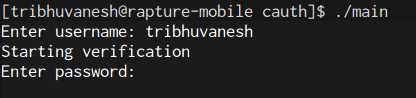
\includegraphics[scale=0.4]{img/login.png}
                \caption{If password matches, proceed to face recognition}
                \label{fig:pwd1}
        \end{subfigure}%
        \begin{subfigure}[b]{0.5\textwidth}
                \centering
                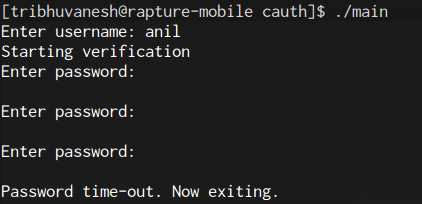
\includegraphics[scale=0.35]{img/login2.png}
                \caption{Otherwise, wait till time-out and exit}
                \label{fig:pwd2}
        \end{subfigure}
        \caption{Conventional username-password login}\label{fig:pwd}
\end{figure}

\subsubsection{ Hard biometrics }
The user-space is representated as a 1-D dimensional space and a normal distribution is plotted expressing the belief of the system of which user is logged in. If the measurement at each iteration produces a certain user-id, it is represented as a univariate normal distribution over this space, with mean $\mu_{1}$ as the user ID and variance $\sigma_{1}^{2}$, an inherent error measure.\\
This \emph{likelihood} $N\left(\mu_{1}, \sigma_{1}^{2}\right)$ coupled with the previous measurement \emph{prior} $N\left(\mu_{2}, \sigma_{2}^{2}\right)$ produces the \emph{posterior} $N\left(\mu, \sigma^{2}\right)$. $\mu$ and $\sigma^{2}$ is calculated as follows:
\begin{align*}
	\mu = \dfrac {\mu_{1}\sigma_{2}^{2} + \mu_{2}\sigma_{1}^{2}} {\sigma_{1}^{2} + \sigma_{2}^{2}}\\[2ex]
	\sigma =\dfrac {1} {\dfrac {1} {\sigma_{1}^{2}}+\dfrac {1} {\sigma_{2}^{2}}}
\end{align*}
The area under the curve between UID $\pm \epsilon$, i.e, the value of the CDF of this univariate distribution determines if the user needs to remain authorized.
\begin{figure}[t]
        \begin{subfigure}[b]{0.5\textwidth}
                \centering
                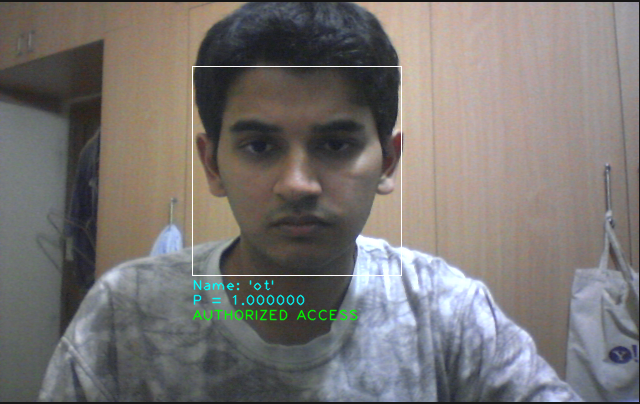
\includegraphics[scale=0.35]{img/hard1.png}
                \caption{As long as authenticated user stays in front of the system, P $>$ 0.9}
                \label{fig:hard1}
        \end{subfigure}%
        \begin{subfigure}[b]{0.5\textwidth}
                \centering
                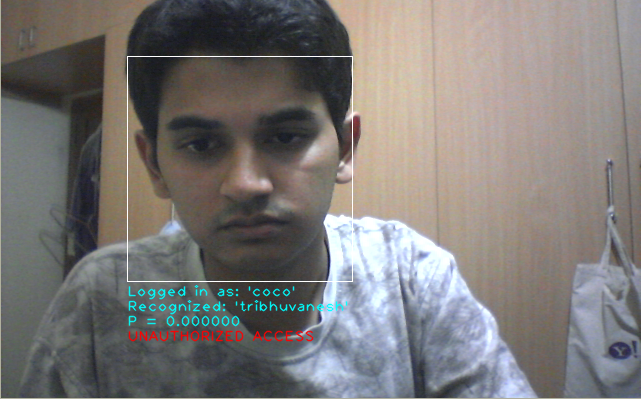
\includegraphics[scale=0.35]{img/unauth3.png}
                \caption{An imposter's probability mass decays and falls to 0}
                \label{fig:pwd2}
        \end{subfigure}
        \caption{Face recognition using hard biometrics}\label{fig:pwd}
\end{figure}
\subsubsection{ Soft biometrics }
The shirt colour, which is determined by a rectangular region just below the detected face is used to determine authorization during the soft biometrics mode. It works as follows:\\[2ex]
\begin{verbatim}
    while(true)
        while(hard_bmt_recog < 0.9)
            frame = get_frame()
            face = preprocess(detect_face(frame))
            hard_bmt_recog = verify(face, face_db)
        // Face recognition gained confidence. Capture soft traits
        soft_template = create_template()
        while(soft_bmt > THRESHOLD)
            soft_details = capture_soft_details()
            soft_bmt = compare(soft_template, soft_details)
\end{verbatim}
% \begin{figure}
% 	\centering
% 		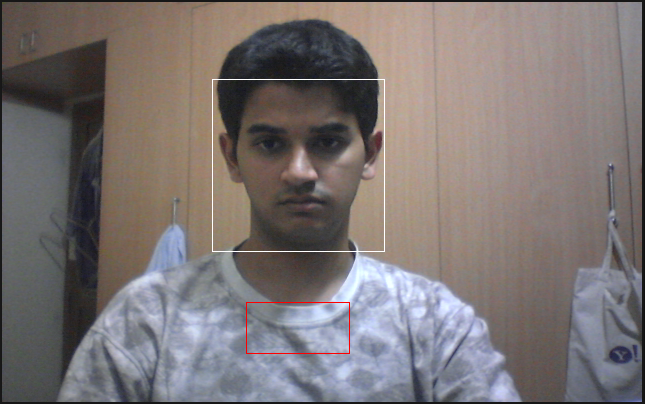
\includegraphics[scale=0.6]{img/soft1.png}
% 	\caption{Soft biometrics - Shirt colour detection}
% \end{figure}

\begin{figure}[h!]
        \begin{subfigure}[b]{0.5\textwidth}
                \centering
                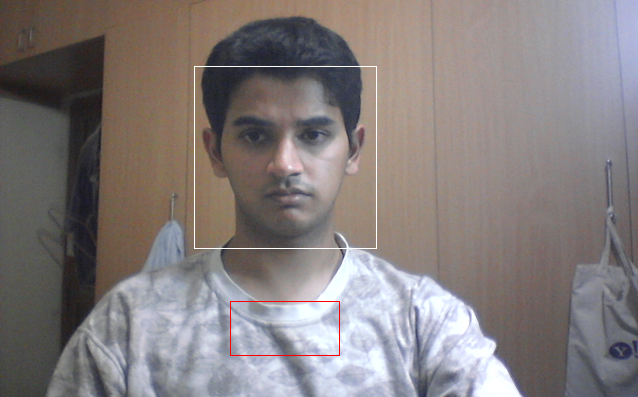
\includegraphics[scale=0.35]{img/soft2.png}
                \caption{Face detection run on the capture image and shirt position detected.}
                \label{fig:soft2_org}
        \end{subfigure}%
        \begin{subfigure}[b]{0.5\textwidth}
                \centering
                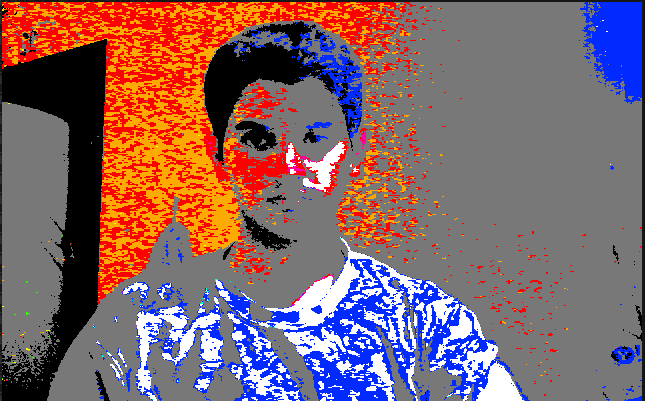
\includegraphics[scale=0.35]{img/soft2_csv.png}
                \caption{Frame converted to CSV, and colour composition of the shirt is calculated}
                \label{fig:soft2_csv}
        \end{subfigure}
        \caption{Authentication using soft biometrics}\label{fig:soft2}
\end{figure}

The soft biometrics template is averaged over frames in $X_{t-k}$ and $X_{t}$ right after the level confidence is highest, that is following the conventional username and password authentication and hard biometrics. Every subsequent k frames are again averaged and compared to the template. 

\begin{figure}[h!]
        \begin{subfigure}[b]{0.5\textwidth}
                \centering
                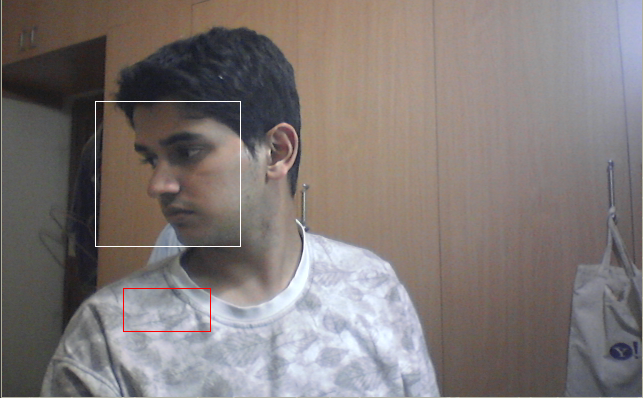
\includegraphics[scale=0.35]{img/soft6.png}
                \caption{Face detection detects with high accuracy even in natural postures}
                \label{fig:soft3_org}
        \end{subfigure}%
        \begin{subfigure}[b]{0.5\textwidth}
                \centering
                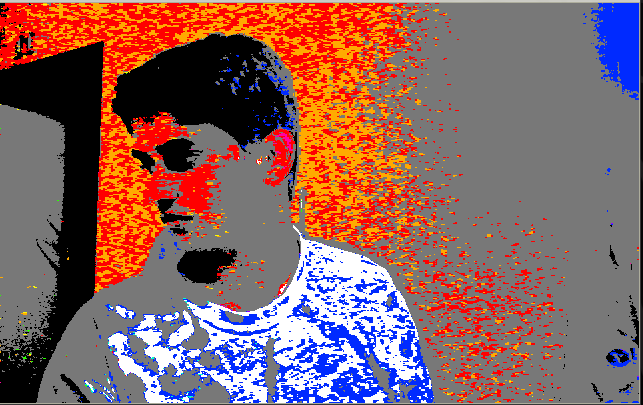
\includegraphics[scale=0.35]{img/soft6_csv.png}
                \caption{Frame converted to CSV, and colour composition of the area is calculated}
                \label{fig:soft3_csv}
        \end{subfigure}
        \caption{Authentication using soft biometrics - Posture}\label{fig:soft3}
\end{figure}

\begin{figure}[h!]
        \begin{subfigure}[b]{0.5\textwidth}
                \centering
                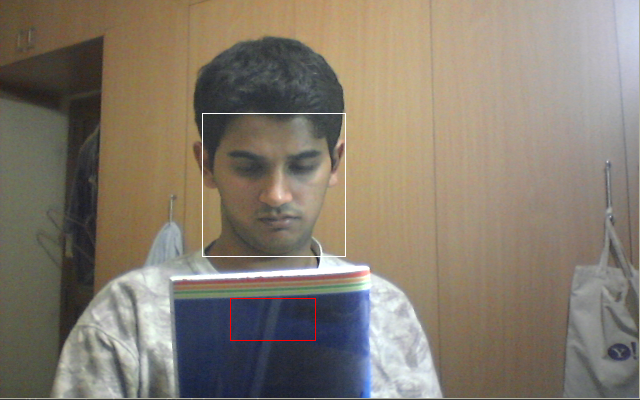
\includegraphics[scale=0.35]{img/soft5.png}
                \caption{Face detection run on the capture image, and new colour composition detected.}
                \label{fig:soft5_org}
        \end{subfigure}%
        \begin{subfigure}[b]{0.5\textwidth}
                \centering
                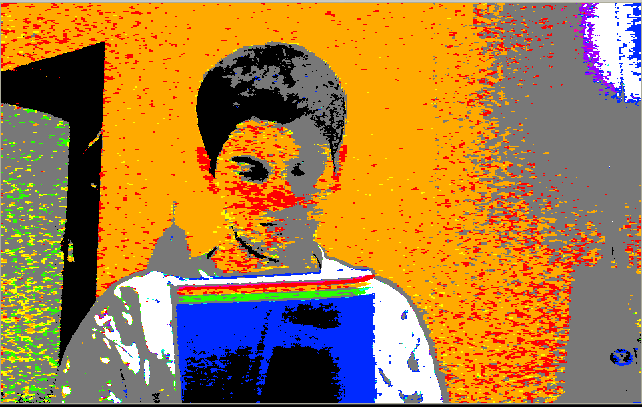
\includegraphics[scale=0.35]{img/soft5_csv.png}
                \caption{Frame converted to CSV, and colour composition of the shirt is calculated}
                \label{fig:soft5_csv}
        \end{subfigure}
        \caption{Authentication using soft biometrics - Occlusion }\label{fig:soft5}
\end{figure}
$\cdot$\\[10ex]
$\cdot$\\[10ex]
\newpage
\section{ Testing }

\subsection{ Unit testing }
The two primary units that comprise the Continuous Authentication system were individually tested under real-world conditions.

\subsubsection{ Face Recognition }
\emph{ Requirement: } Faces should be accurately recognized\\
\emph{ Test: } A burst of 200 frames were collected with the user posing naturally with head movement\\
\emph{ Result: } An accuracy of 94\% was achieved.\\

\subsubsection{ Soft bio-metrics }
\emph{ Requirement: } The soft-biometrics captured should not vary by large from the initial captured template\\
\emph{ Test: } A burst of 200 frames was used with the user performing extreme movements\\
\emph{ Result: } An accuracy of 78\% was achieved\\

\subsection{ Performance testing } 
\emph{ Requirement: } The Continuous Authentication system should be able to meet real-time requirements on a system\\
\emph{ Test: } The code was tested on two systems - one with a Core 2 Duo processor at 3.0Ghz, and the other with a Core i5 processor at 2.66 Ghz\\
\emph{ Result: } The real time requirements was easily met on the Core i5 system, and the Core 2 Duo system, but with a minor lag\\

\subsection{ Security testing}
\emph{ Requirement: } One should not be able to log in without the right credentials, or be able to reverse engineer\\
\emph{ Test: } The passwords stored in the database should not be readable\\
\emph{ Result: } Since the SHA1 hashes of the users were stored in the database, it's harmless even if one tries to retrieve it\\

\subsection{ Compatibility testing }
\emph{ Requirement: } The CA system should be compatible with all the latest versions of the libraries used\\
\emph{ Test: } The code was compiled and executed on g++ 4.5-2.7, OpenCV versions 2.1-2.3 and 2 distributions of Linux\\
\emph{ Result: } The code successfully compiled and executed on all the above versions\\

\subsection{ Load Testing }
\emph{ Requirement: } The CA system should be able to lock-on on one sigle person and perform verification \\
\emph{ Test: } The system was tested with multiple people in the frame\\
\emph{ Result: } A lock-on was always performed on the largest-detected face in the frame\\

\subsection{ Integration testing}
\emph{ Requirement: } By integrating the two main components of Continuous Authentication, the system should successfully switch between them as and when needed\\
\emph{ Test: } A 10 minute run was conducted under real-world conditions\\
\emph{ Result: } The soft-biometrics mode was successfully able to switch to face recognition mode when confidence dropped below a certain threshold\\

\subsection{ System testing }
\emph{ Requirement: } A tail-gating unauthorized user should not be able to gain access for over 3-5 seconds\\
\emph{ Test: } A 10 minute run was conducted with the user and an imposter switching a number of times\\
\emph{ Result: } The imposter was able to gain access for over 5 seconds 2 times out of the 10 switches performed\\

\newpage

\section{ Results }
The Continuous Authentication system was tested using 12 users in total, with 10 of those users having credentials registered in the database. Each user was logged in for a certain period in time, while the others tail-gated the authorized user. 

\begin{figure}[b]
	\caption{Time taken - Face recognition vs. Soft biometrics}
	\centering
		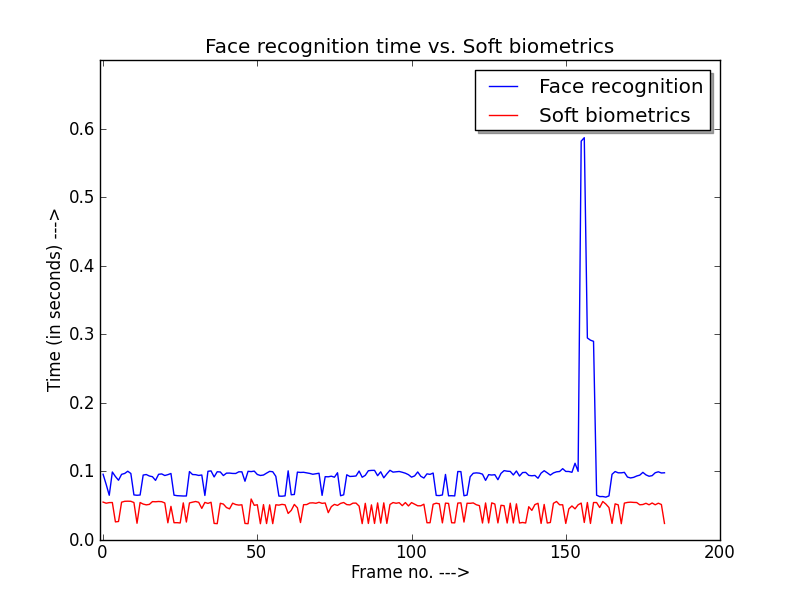
\includegraphics[scale=0.6]{img/face_vs_soft.png}
\end{figure}

\begin{figure}
	\caption{Face recognition accuracy - 94\%}
	\centering
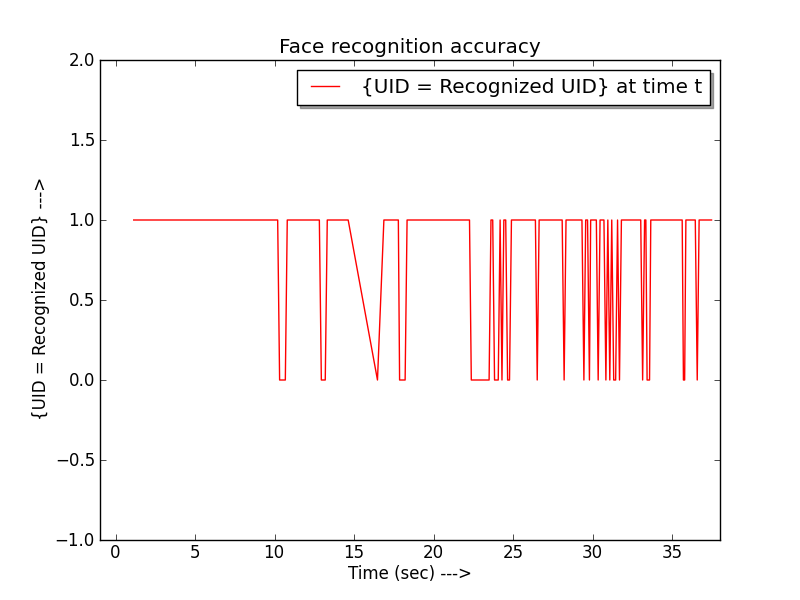
\includegraphics[scale=0.6]{img/face_rec_accuracy.png}
\end{figure}
\begin{figure}
	\caption{Mean vs. Recognized vs. Authorized}
	\centering
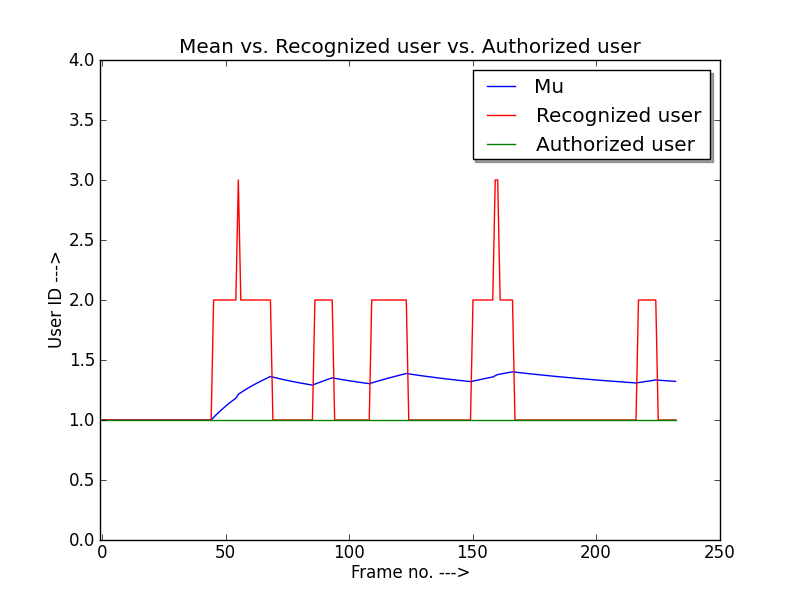
\includegraphics[scale=0.6]{img/mu_nearest_uid.png}
\end{figure}

\begin{figure}
	\caption{Initial uncertainity of user}
	\centering
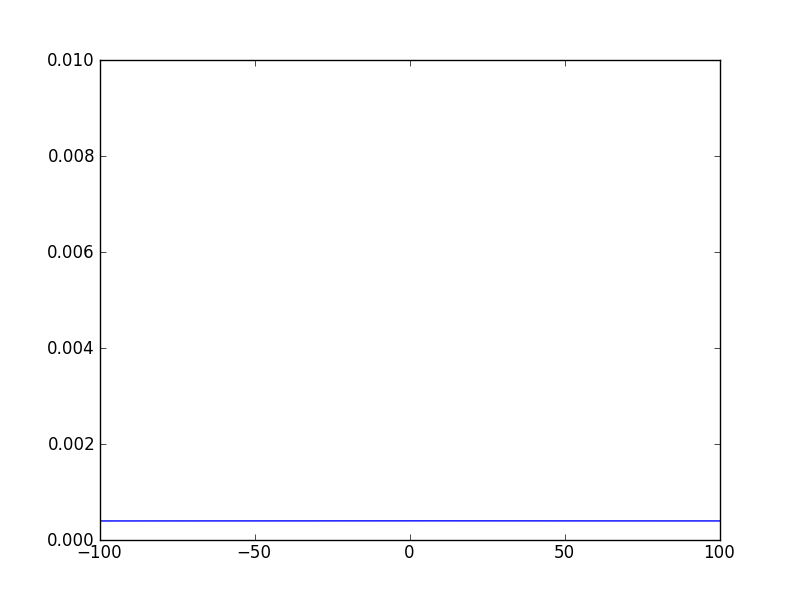
\includegraphics[scale=0.6]{img/mu_sig1.png}
\end{figure}

\begin{figure}
	\caption{Variance decreases in the subsequent frames if the authenticated user is present}
	\centering
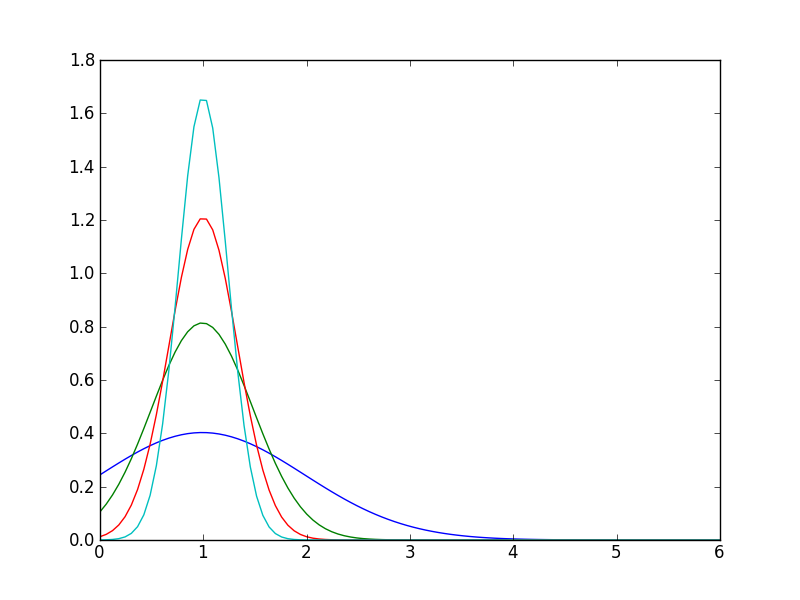
\includegraphics[scale=0.6]{img/mus_sig3.png}
\end{figure}
\begin{figure}
	\caption{Variance continues decreasing. Area under curve increases}
	\centering
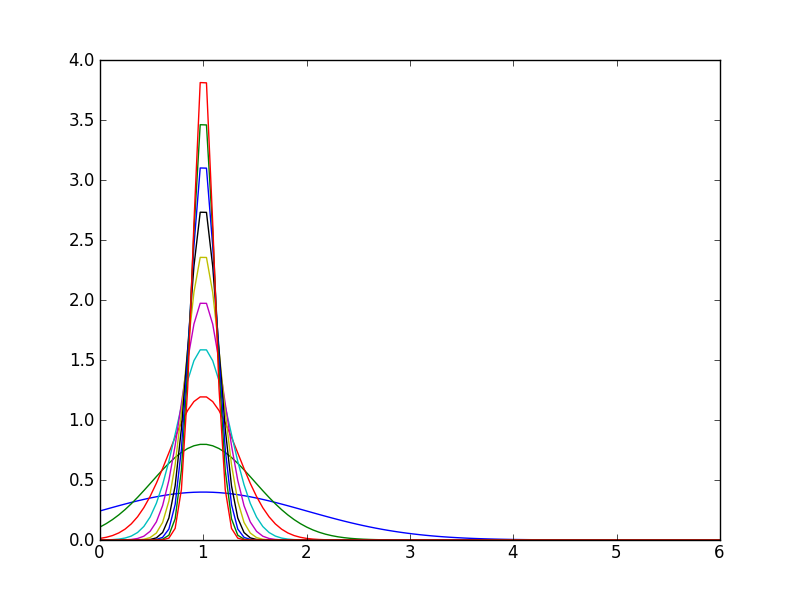
\includegraphics[scale=0.6]{img/mus_sig4.png}
\end{figure}

\begin{figure}
	\caption{Mean shifts as user changes}
	\centering
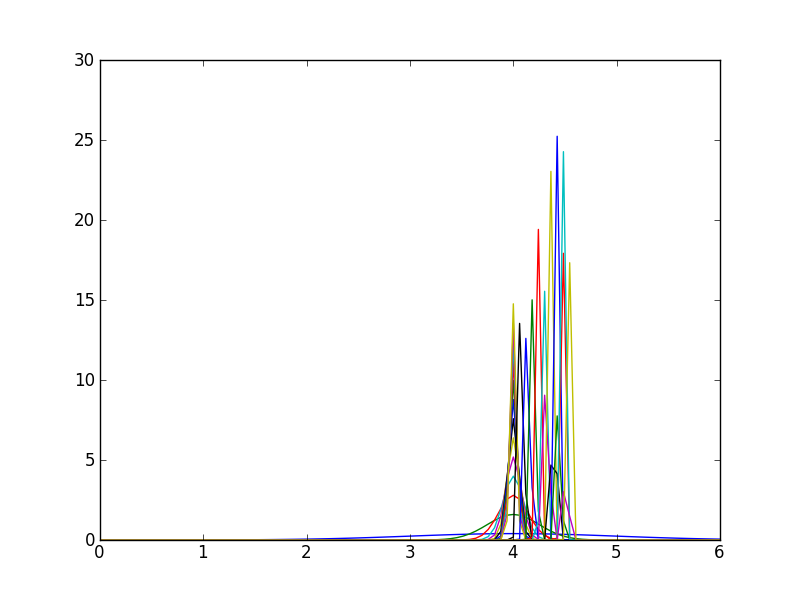
\includegraphics[scale=0.6]{img/mu_sig5.png}
\end{figure}

\begin{figure}
	\caption{Magnified version of previous figure}
	\centering
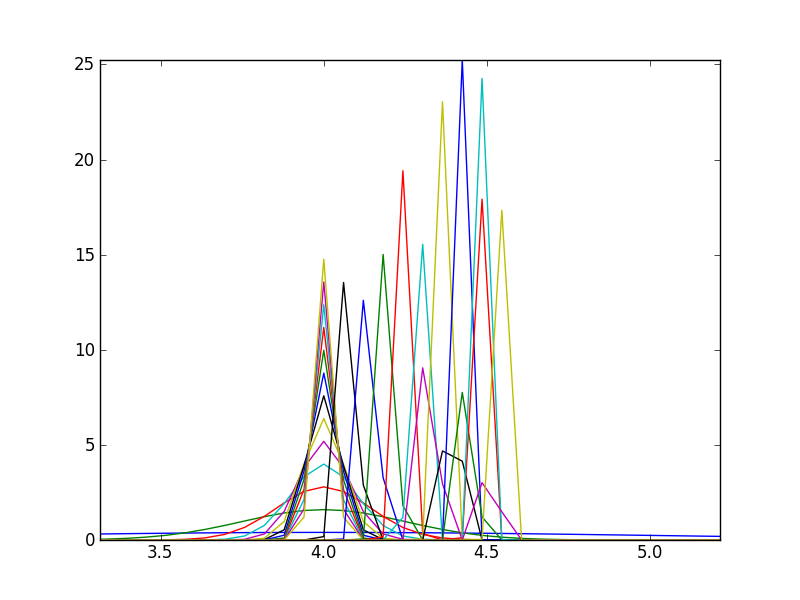
\includegraphics[scale=0.6]{img/mus_sig5.png}
\end{figure}

$\cdot$\\[10ex]
$\cdot$\\[10ex]
$\cdot$\\[10ex]
$\cdot$\\[10ex]
\newpage
\section{ Conclusion and Future Enhancements }
\subsection {Conclusion}
Need for biometric authentication arose from the fact that other security measures such as password and/or a smart ID card are prone to theft or loss. Biometrics depend on utilising features a user already possesses, that can uniquely identify a user atleast for a given session. However, using biometric identification has its downfalls. Since the characteristic of biometric traits is that they are not secretive, unlike a password, they can be gathered anywhere by an imposter and reconstructed for the authentication system to gain access. For example, a fingerprint left behind on some surface, can be picked up by imposters and reconstructed in front of the sensors. Even for face recognition systems, it is possible to fool the system by showing a photograph of the user or manipulating the video feed of the system. Countermeasures exist for such instances, such as, 3d reconstruction of face from more than two cameras or ensuring that the video feed cannot be manipulated. However, these measures make it a costly solution. Therefore, it can be concluded that biometric mode of authentication should be used more as a support system along with password/ smartID systems, to strengthen the authentication process, rather than a standalone mode of authentication.   

\subsection {Future Enhancements}
The following can be implemented in the future to enhance this system:
\begin{itemize}
\item Support for multiple users sharing a certain account; this may require a "biometric handoff" to occur between users.
\item Improve accuracy of face recognition under varied lighting conditions by implementing recognition using a different approach such as fuzzy logic.
\item Make provision for recognizing any kind of tampering occuring to the video feed, so as to prevent authenticating imposters. This can be done by restricting access to the webcam feed via parameters that define access to it.
\end{itemize}


\section{ References }
\begin{thebibliography}{77}
\bibitem{Turk91} M. Turk and A. Pentland.
"Face recognition using eigenfaces."
\emph{Proc. IEEE Conference on Computer Vision and Pattern Recognition.} pp. 586-591.

\bibitem{Viola01}Paul Viola, Michael Jones.
"Robust Real-time Object Detection."
\emph{Second International Workshop on Statistical and Computational Theories of Vision - Modeling, Learning, Computing, and Sampling (Vancouver, Canada)}, July 13, 2001.

\bibitem{Niin10} Niinuma, K., Unsang Park, Fujitsu Labs. Ltd., Kawasaki, Japani, A.K. Jain
"Soft Biometric Traits for Continuous User Authentication" 
\emph{Information Forensics and Security, IEEE Transactions on}, 2010

\bibitem{Jain04}A.K. Jain, S.C. Dass, K. Nandakumar.
"Soft Biometric Traits for Personal Recognition Systems."
\emph{International Conference on Biometric Authentication}, 2004.

\bibitem{Klos00}Andrew J. Klosterman, Gregory R. Ganger.
"Secure Continuous Biometric-Enhanced Authentication", 
Carnegie Mellon University, Tech. Rep. CMU-CS-00-134, 2000.

\bibitem{Jain204}A. K. Jain, S. C. Dass, and K. Nandakumar,
“Can soft biometric traits assist user recognition?”,
Proc. SPIE, vol. 5404, pp. 561–572, 2004.

\bibitem{libsvm}Chang, Chih-Chung and Lin, Chih-Jen,
LIBSVM: A library for support vector machines,
\emph{ACM Transactions on Intelligent Systems and Technology}
available at \url{http://www.csie.ntu.edu.tw/~cjlin/libsvm}

\bibitem{servo}How face detection works,
\href{http://www.servomagazine.com/}{SERVO Magazine}, 2007

\bibitem{ann99}Anne Adams and Martina Angela Sasse.
Dec,1999/Vol.42.No.12, Communications ofthe ACM,
P40-Parker, D.B. Restating the foundation of information security-- In G.C.
Gable and W.J. Caelli, Eds., IT Security: The Need for International Cooperation.
Elsevier Science Publishers, Holland, 1992

\bibitem{war02} Ware, Karl.
Biometrics and strong authentication McGraw-Hill Osborne

\bibitem{john03}John Woodward, Nicholas M. Orlans, Peter T. Higgins.
Biometrics and strong authentication,McGraw-Hill Inc, 2003

\bibitem{bert96}A. Bertillon,
Signaletic Instructions including the theory and practice of Anthropometrical Identification, R.W.
McClaughry Translation, The Werner Company, 1896.

\bibitem{way97}J. L. Wayman,
“Large-scale Civilian Biometric Systems - Issues and Feasibility,” in Proceedings of Card Tech /
Secur Tech ID, 1997.

\bibitem{mon00}
F. Monrose and A. D. Rubin, 
“Keystroke dynamics as biometrics for authentication,” 
Future Generation Comput. Syst., vol. 16, pp.351–359, 2000.

\bibitem{turk03}
A. Altinok and M. Turk, 
“Temporal integration for continuous multi-modal biometrics,”
in Proc. Workshop on Multimodal User Authentication, 2003, pp. 131–137.

\bibitem{sim07}
T. Sim, S. Zhang, R. Janakiraman, and S. Kumar, 
“Continuous verification using multimodal biometrics,” 
IEEE Trans. Pattern Anal. Mach. Intell., vol. 29, no. 4, pp. 687–700, Apr. 2007.

\bibitem{azz08}
A. Azzini, S. Marrara, R. Sassi, and F. Scotti, “A fuzzy approach to
multimodal biometric continuous authentication,” Fuzzy Optimal De-
cision Making, vol. 7, pp. 243–256, 2008.
\bibitem{azz082}
A. Azzini and S. Marrara, “Impostor users discovery using a multi-
modal biometric continuous authentication fuzzy system,” Lecture
Notes in Artificial Intelligence, vol. 5178, pp. 371–378, 2008.
\bibitem{kang06}
H.-B. Kang and M.-H. Ju, “Multi-modal feature integration for secure
authentication,” in Proc. Int. Conf. Intelligent Computing, 2006, pp.
1191–1200.
\bibitem{car03}
C. Carrillo, “Continuous Biometric Authentication for Authorized Air-
craft Personnel: A Proposed Design,” Master’s thesis, Naval Postgrad-
uate School, Monterey, CA, 2003.

\end{thebibliography}


\section{ Appendix }
\subsection{ Screen Snapshots}
\begin{figure}
	\caption{Occlusion is dealt by using hard biometrics}
	\centering
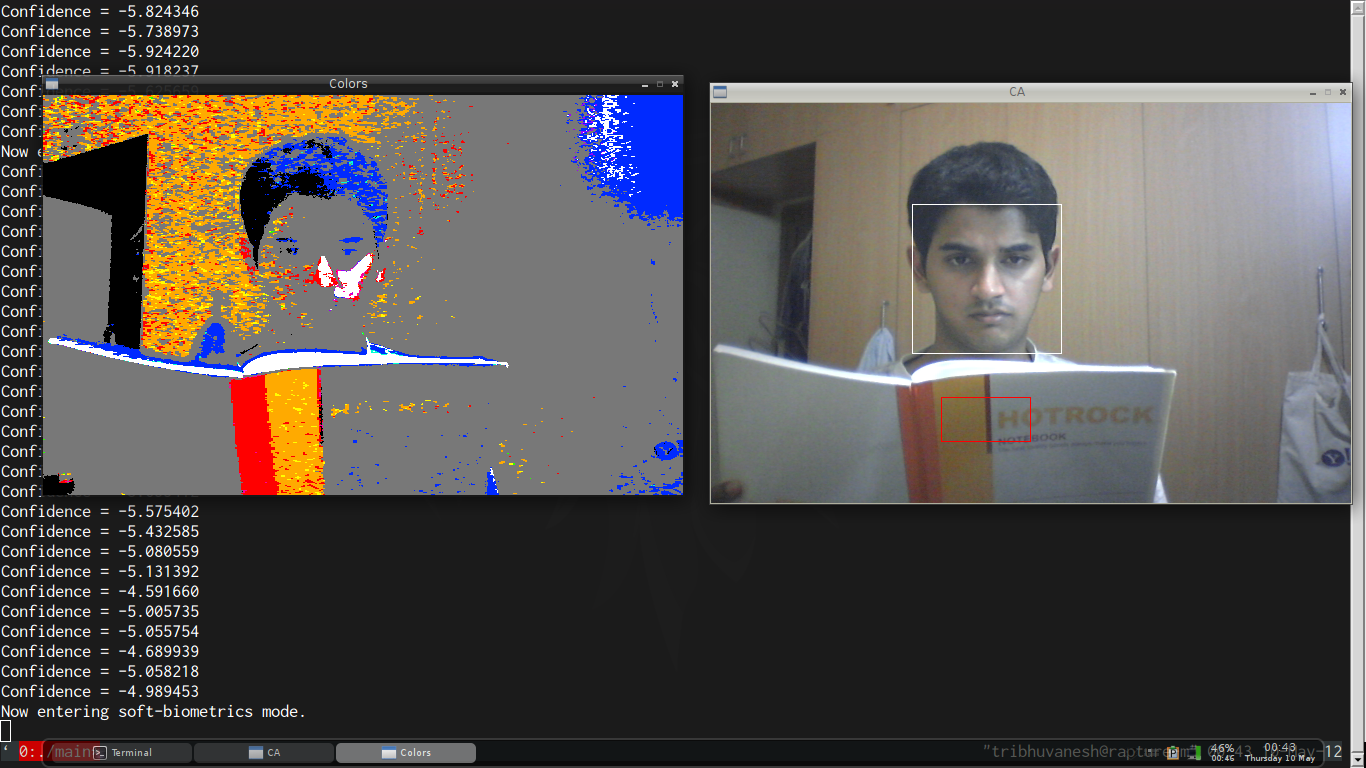
\includegraphics[scale=0.3]{img/soft4.png}
\end{figure}

\begin{figure}
	\caption{Unauthorized. Lock-down}
	\centering
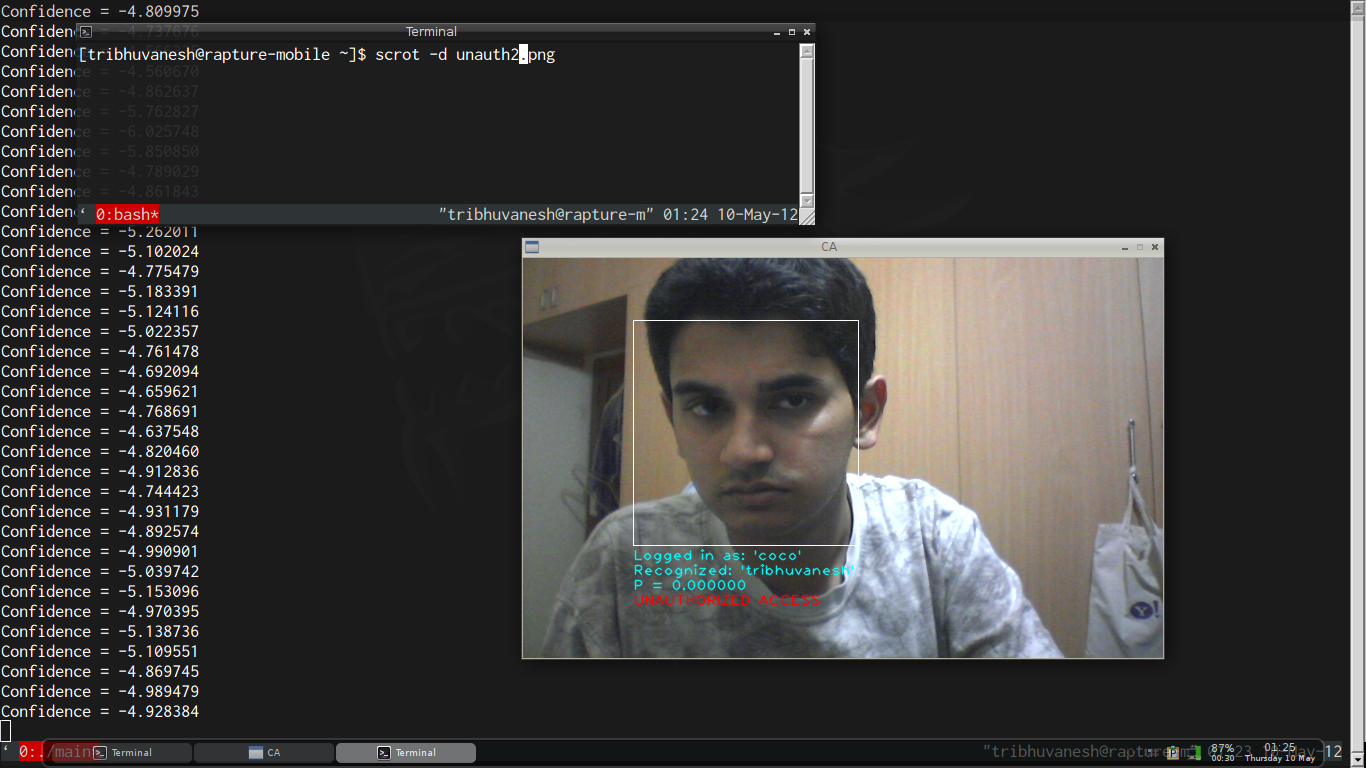
\includegraphics[scale=0.3]{img/unauth2.png}
\end{figure}

\begin{figure}
	\caption{Authorized. Authenticated mode.}
	\centering
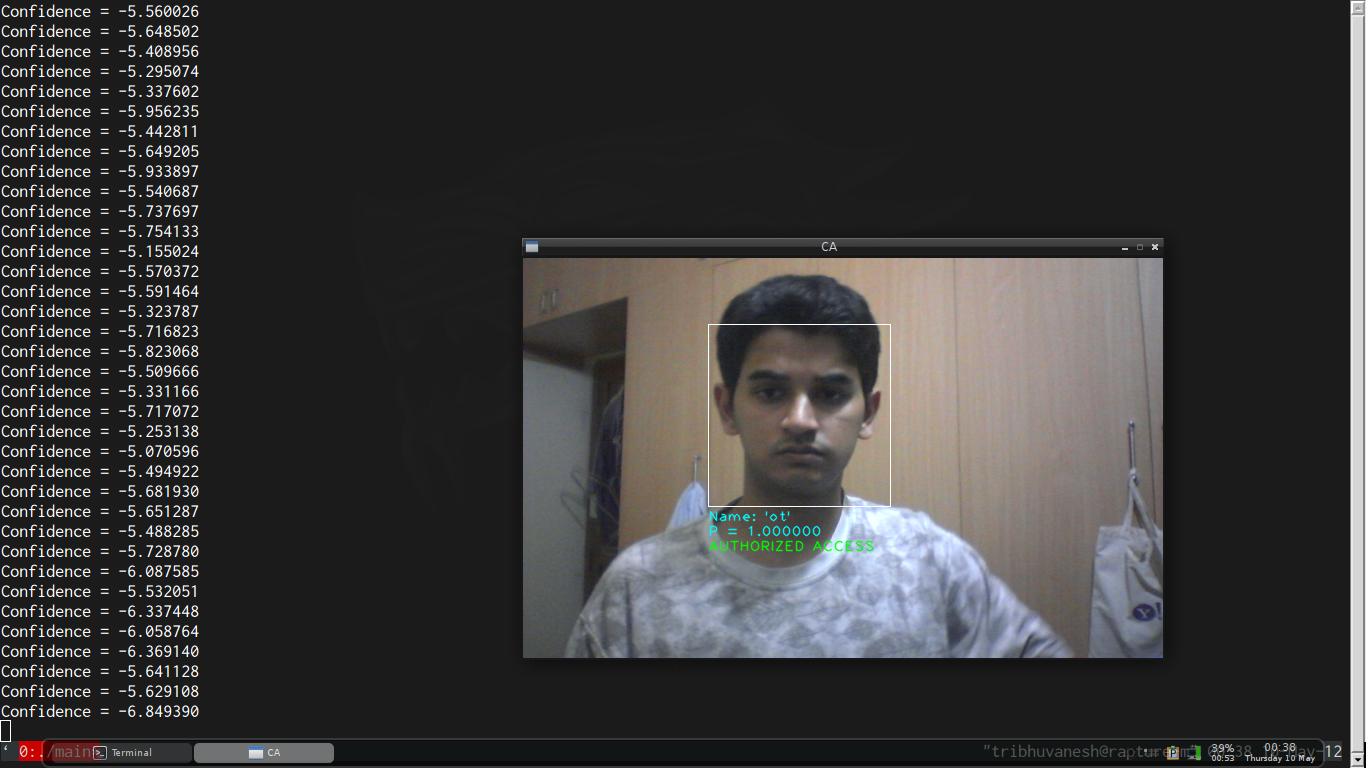
\includegraphics[scale=0.3]{img/hard2.png}
\end{figure}

\begin{figure}
	\caption{Average image obtained after training. Deviations calculated later from this image to obtain eigenvectors.}
	\centering
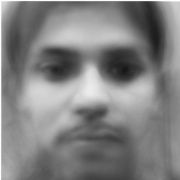
\includegraphics[scale=1]{img/avg_image.jpeg}
\end{figure}

\begin{figure}
	\caption{Eigenvectors}
	\centering
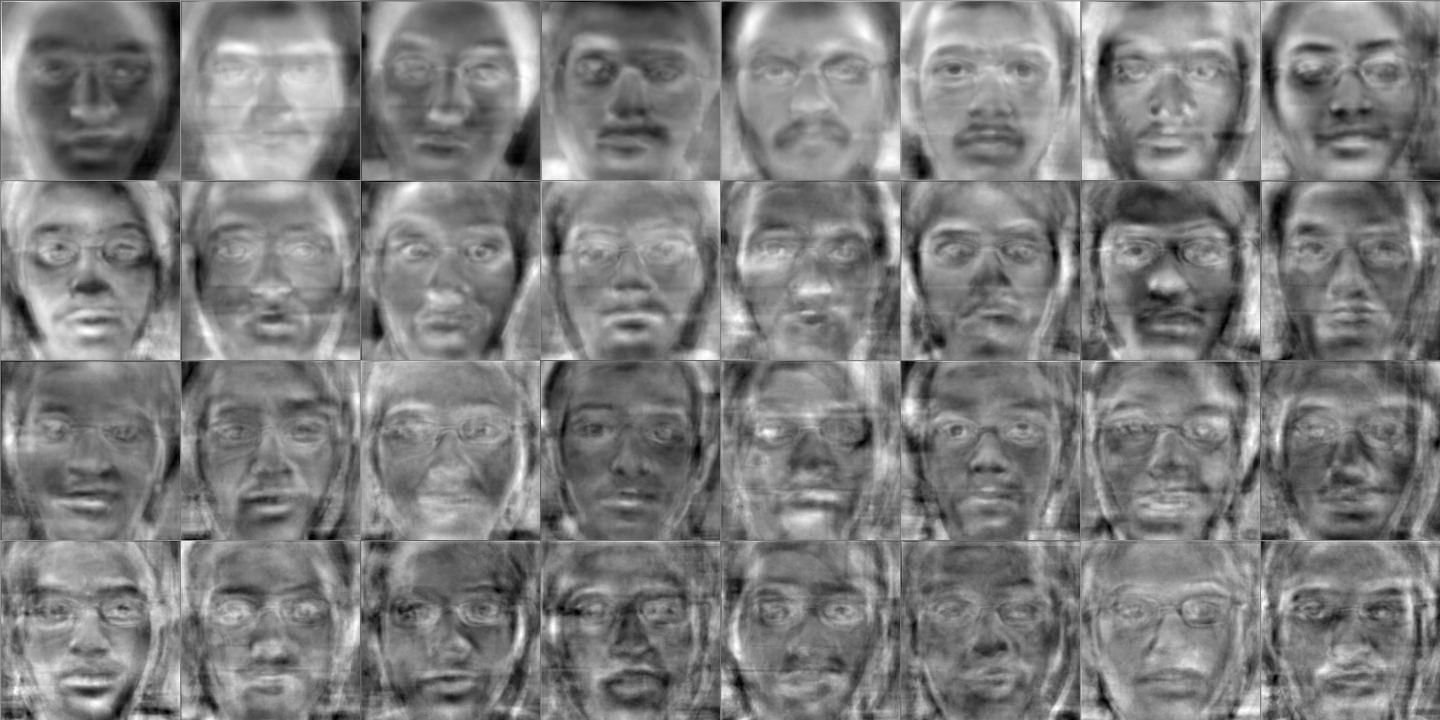
\includegraphics[scale=0.2]{img/eigen.png}
\end{figure}
% \section{ Applications }  
\end{document}				% REQUIRED

